\documentclass[11pt,letterpaper]{article}

\usepackage{fontspec}
\setmainfont{LiberationSans}[Path=/usr/share/fonts/liberation/, Extension=.ttf, UprightFont=*-Regular, BoldFont=*-Bold, ItalicFont=*-Italic, BoldItalicFont=*-BoldItalic]
\usepackage[spanish,es-noshorthands,es-tabla,es-noitemize]{babel}
\usepackage[letterpaper,top=2cm,bottom=2cm,left=2cm,right=2cm]{geometry}
\usepackage{graphicx}
\usepackage{xcolor}
\usepackage{tikz}
\usetikzlibrary{positioning,arrows.meta}
\usepackage{tabularx}
\usepackage{array}
\usepackage{enumitem}
\usepackage{titlesec}
\usepackage{caption}
\usepackage[hidelinks]{hyperref}
\usepackage{xurl}
\urlstyle{same}

\definecolor{cpucol}{HTML}{E4E6EA}
\definecolor{pciecol}{HTML}{F6D7B0}
\definecolor{gpucol}{HTML}{C9E8D2}

\titleformat{\section}[block]{\centering\bfseries\fontsize{16}{19}\selectfont}{\thesection.}{0.4em}{}
\titleformat{\subsection}{\bfseries\fontsize{14}{17}\selectfont}{\thesubsection}{0.6em}{}
\titlespacing*{\section}{0pt}{7pt}{3pt}
\titlespacing*{\subsection}{0pt}{5pt}{2pt}
\setlist{nosep,leftmargin=1.3em,topsep=2pt}
\setlength{\parindent}{0pt}
\setlength{\parskip}{3.5pt}
\captionsetup{labelsep=period,skip=3pt}
\setlength{\textfloatsep}{6pt}
\setlength{\intextsep}{5pt}
\renewcommand{\arraystretch}{1.08}
\pagestyle{plain}

\begin{document}

\begin{titlepage}
  \centering
  
\includegraphics[width=3.4cm]{logo-uvg.png}\par
  \vspace{0.8cm}
  Universidad del Valle de Guatemala\par
  CC3069 Computación Paralela y Distribuida, sección 20\par
  Ing. Juan Luis García\par
  \vspace{4.5cm}
  {\bfseries\fontsize{16}{19}\selectfont Caso 1: Radiografías que no esperan\par}
  \vspace{0.6cm}
  Caso práctico: CUDA en el mundo real\par
  Informe final\par
  \vspace{4.5cm}
  Grupo 1\par
  \vspace{0.3cm}
  \begin{tabular}{ll}
    Diego López     & 23747 \\
    Nicolás Concuá  & 23197 \\
    Esteban Cárcamo & 23016 \\
  \end{tabular}\par
  \vfill
  Guatemala, 11 de noviembre de 2026\par
\end{titlepage}

\setcounter{page}{1}

\section{Problema y usuario}

El Instituto Guatemalteco de Seguridad Social (IGSS) realizó 895\,987 estudios de rayos X en 2024, unos 2\,455 al día (IGSS, 2025). Solo el hospital de Escuintla registra un promedio preliminar de 5\,981 estudios al mes, unos 197 al día (IGSS, 2026). Cuando se leen por orden de llegada, la placa de un paciente con edema pulmonar puede quedar detrás de decenas de estudios normales, aunque el edema pulmonar agudo es una emergencia con una mortalidad hospitalaria de 11,4\,\% en una cohorte de urgencias (Cosentini et al., 2009). La decisión que depende de esto es qué placa se abre primero. En un estudio con 15\,887 radiografías, la priorización automática redujo en simulación la demora media de los hallazgos críticos de 11,2 a 2,7 días (Annarumma et al., 2019). Este trabajo asigna a cada placa un puntaje de urgencia y ordena la cola. El sistema prioriza y no diagnostica: el radiólogo sigue leyendo todos los estudios.

\section{Datos}

Se usó un subconjunto de NIH ChestX-ray14 (Wang et al., 2017). No se encontró una cifra pública del número de radiólogos del IGSS ni un conjunto de placas guatemaltecas de libre acceso, por lo que los datos clínicos son del NIH y las cifras de volumen son del IGSS.

\begin{table}[h]
\centering
\caption{Conjunto de datos utilizado.}
\begin{tabularx}{\linewidth}{|l|X|}
\hline
Fuente & NIH Clinical Center, \url{https://nihcc.app.box.com/v/ChestXray-NIHCC}. Etiquetas y particiones tomadas del espejo \texttt{alkzar90/NIH-Chest-X-ray-dataset} de Hugging Face \\ \hline
Tamaño & 44\,999 radiografías de 11\,558 pacientes (archivos images\_001 a images\_005): 17,7 GB comprimidos y 17,7 GB en PNG \\ \hline
Formato & PNG de 1024 × 1024 píxeles; CSV con 14 hallazgos; 27\,090 proyecciones PA y 17\,909 AP \\ \hline
Licencia & Uso sin restricciones, con enlace al NIH, cita a Wang et al. (2017) y reconocimiento al NIH Clinical Center \\ \hline
\end{tabularx}
\end{table}

La preparación verificó la integridad de los archivos, el tamaño de cada imagen y su correspondencia con el CSV: no hubo imágenes ilegibles ni sin etiqueta. Se detectaron 421 PNG en RGBA, todos con R = G = B y alfa opaco, por lo que la conversión a gris es exacta. La lista fija de imágenes es la misma para ambas versiones. La precisión se evaluó solo con las 7\,724 imágenes de la partición oficial de prueba.

\section{Solución en CPU y en GPU}

Ambas versiones comparten en \texttt{comun/tarea.py} la lista de imágenes, la decodificación, el recorte, la reducción, la normalización, el modelo y el puntaje. Cada placa se decodifica con OpenCV (Bradski, 2000), se recorta al centro, se reduce a 224 × 224 por promedio de área, se normaliza a [−1024, 1024] y pasa por DenseNet-121 (Huang et al., 2017) con los pesos \texttt{densenet121-res224-all} de TorchXRayVision (Cohen et al., 2022), en FP32. El puntaje es la mayor probabilidad entre neumotórax, edema, neumonía, derrame y consolidación. La versión de CPU usa NumPy (Harris et al., 2020) y PyTorch (Paszke et al., 2019). La de GPU usa PyTorch con cuDNN, con TF32 apagado, y un kernel propio en CuPy (Okuta et al., 2017).

\begin{figure}[h]
\centering
\begin{tikzpicture}[
  box/.style={draw=black!55, rounded corners=2pt, align=center, font=\scriptsize,
              minimum height=1.2cm, text width=1.95cm, inner sep=2pt},
  arr/.style={-{Stealth[length=4pt]}, thick, black!60},
  node distance=0.3cm]
  \node[box, fill=cpucol]               (a) {Leer PNG\\de disco\\\textit{(CPU)}};
  \node[box, fill=cpucol,  right=of a]  (b) {Decodificar\\PNG\\\textit{(CPU, hilos)}};
  \node[box, fill=pciecol, right=of b]  (c) {Copia a GPU\\en uint8\\\textit{(PCIe)}};
  \node[box, fill=gpucol,  right=of c]  (d) {Recorte,\\224 × 224 y\\normalización\\\textit{(kernel CuPy)}};
  \node[box, fill=gpucol,  right=of d]  (e) {DenseNet-121\\por lotes\\\textit{(cuDNN)}};
  \node[box, fill=gpucol,  right=of e]  (f) {Puntaje: máx.\\de hallazgos\\críticos\\\textit{(GPU)}};
  \node[box, fill=gpucol,  right=of f]  (g) {Cola\\ordenada\\\textit{(GPU)}};
  \foreach \x/\y in {a/b,b/c,c/d,d/e,e/f,f/g} \draw[arr] (\x) -- (\y);
\end{tikzpicture}
\caption{Etapas de la versión GPU: en gris, la CPU; en naranja, la transferencia, y en verde, la GPU.}
\end{figure}

El kernel usa un hilo por píxel de salida: 50\,176 por imagen, en bloques de 16 × 16, con una imagen por bloque en el eje z. Cada hilo promedia una caja de 5 × 5 a 6 × 6 píxeles de entrada y aplica la normalización. Las imágenes se copian en uint8 desde memoria fijada y se procesan en lotes de 64, de modo que nunca se cargan los 45 GB decodificados. Las dos colas resultan equivalentes: la diferencia máxima de puntaje es 2 × 10\textsuperscript{−6}, las 100 placas más urgentes coinciden, ninguna placa se mueve más de 2 posiciones y el AUC es idéntico.

\section{Mediciones}

Ambas versiones corrieron en la misma laptop: Intel Core i9-13980HX, 15 GB de RAM y NVIDIA GeForce RTX 4050 Laptop con 6 GB de VRAM, PyTorch 2.15.0 con CUDA 13.2. Se reporta la mediana de cinco corridas tras una de calentamiento, sin contar la carga del modelo. Las etapas de la GPU se midieron con eventos de CUDA y las de la CPU con \texttt{perf\_counter}. La CPU usó su mejor configuración de un barrido: 8 hilos en núcleos P, a 31,1 img/s, frente a 14,9 img/s con 32 hilos.

\begin{table}[h]
\centering
\caption{Tiempo por etapa con 44\,999 imágenes, en segundos.}
\begin{tabular}{|l|r|r|r|r|r|}
\hline
Etapa & CPU & \% & GPU & \% & Speedup \\ \hline
Lectura & 19,11 & 1,3 & 18,42 & 10,6 & 1,0× \\ \hline
Decodificación & 53,48 & 3,7 & 27,60 & 15,9 & 1,9× \\ \hline
Copia a la GPU & — & — & 3,96 & 2,3 & — \\ \hline
Preprocesado & 79,25 & 5,5 & 0,36 & 0,2 & 219,2× \\ \hline
Inferencia & 1\,293,66 & 89,5 & 122,82 & 70,9 & 10,5× \\ \hline
Puntaje y orden & 0,09 & 0,0 & 0,14 & 0,1 & 0,7× \\ \hline
Total & 1\,445,8 & 100 & 173,3 & 100 & 8,3× \\ \hline
\end{tabular}
\end{table}

T\textsubscript{CPU} fue 1\,445,8 s (24,1 min, 31,1 img/s) y T\textsubscript{GPU} fue 173,3 s (2,9 min, 259,7 img/s), con un speedup de 8,3×. La transferencia tomó 3,96 s, el 2,3 \% de T\textsubscript{GPU}: 43,9 GiB a 11,9 GB/s. La VRAM pico fue de 2,5 GB.

\begin{table}[h]
\centering
\caption{Variantes de la versión GPU con 44\,999 imágenes.}
\begin{tabularx}{\linewidth}{|l|r|r|X|}
\hline
Variante & img/s & T (s) & Observación \\ \hline
Base: uint8, kernel, fijada, lote 64 & 259,7 & 173,3 & Copia de 3,96 s \\ \hline
Solapado de decodificación y GPU & 322,0 & 139,8 & 10,3× frente a la CPU \\ \hline
Copia en float32 & 238,7 & 188,5 & Copia de 15,33 s y 175,8 GiB \\ \hline
Memoria paginable & 258,6 & 174,0 & Copia de 6,75 s, a 7,0 GB/s \\ \hline
Preprocesado en PyTorch & 255,8 & 175,9 & 2,65 s; el kernel es 7,3× más rápido \\ \hline
Lote de 32 / de 128 & 263,4 / 265,2 & 170,8 / 169,7 & VRAM de 1,8 / 4,0 GB \\ \hline
Mismos 8 hilos de la CPU & 226,8 & 198,4 & Decodificación de 53,6 s; 7,3× \\ \hline
\end{tabularx}
\end{table}

\section{Análisis}

\begin{figure}[h]
\centering
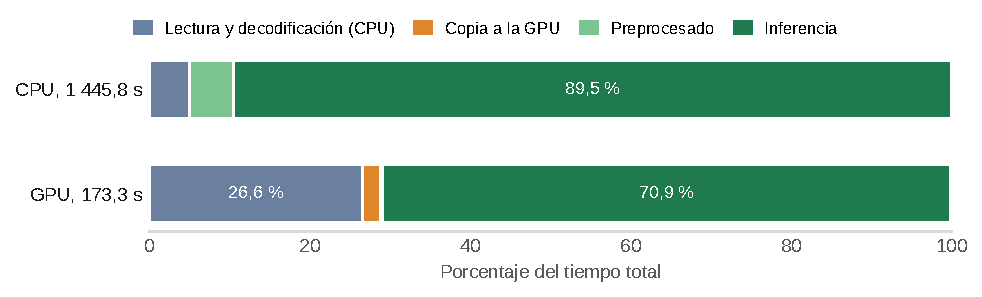
\includegraphics[width=0.94\linewidth]{figuras/etapas.pdf}
\caption{Distribución del tiempo por etapa: la GPU desplaza el peso hacia la lectura y la decodificación.}
\end{figure}

En la CPU, el cuello de botella es la inferencia (89,5 \%, Figura 2). En la GPU sigue siendo la etapa mayor (70,9 \%), pero lectura y decodificación pasan de 5,0 \% a 26,6 \%. La copia no es el problema: enviar uint8 en vez de float32 la redujo 3,9 veces.

Lectura y decodificación son la parte que la GPU no acelera: 72,6 s, una fracción s = 5,02 \%. Por la Ley de Amdahl, el speedup máximo es 1/s = 19,9×. Con el resto acelerado 10,5×, la ley predice 1/(s + (1 − s)/10,5) = 7,1×. La variante con los mismos 8 hilos midió 7,3×, lo que confirma el modelo. El total de 8,3× es mayor porque en la versión GPU la CPU queda libre para decodificar con 32 hilos. El solapado oculta parte de esa fracción y llega a 10,3×. Avanzar más exigiría decodificar en la GPU o guardar las imágenes ya decodificadas.

Con 10 veces más datos (449\,990 imágenes), el tiempo escalaría linealmente a 4,02 h en CPU y 28,9 min en GPU. La RAM y la VRAM no cambian porque se procesa por lotes. Esta extrapolación es optimista en la lectura: 177 GB ya no aprovecharían la caché del sistema operativo, así que el disco pesaría más.

Dos resultados no estaban previstos. El 37 \% de los pesos eran números desnormalizados, que en x86 siguen un camino lento: pasarlos a cero duplicó la velocidad de la CPU (14,6 a 31,1 img/s) sin cambiar la salida, y no afectó a la GPU. Además, en este procesador híbrido más hilos no significaron más velocidad, porque los núcleos P esperan a los núcleos E en cada sincronización.

\section{Resultado e impacto}

Para medir la utilidad de la cola se simularon 5\,000 colas de 300 placas tomadas de la partición de prueba, donde el 32 \% tiene algún hallazgo crítico. Por orden de llegada, la posición media es 150,5 (Figura 3).

\begin{figure}[h]
\centering
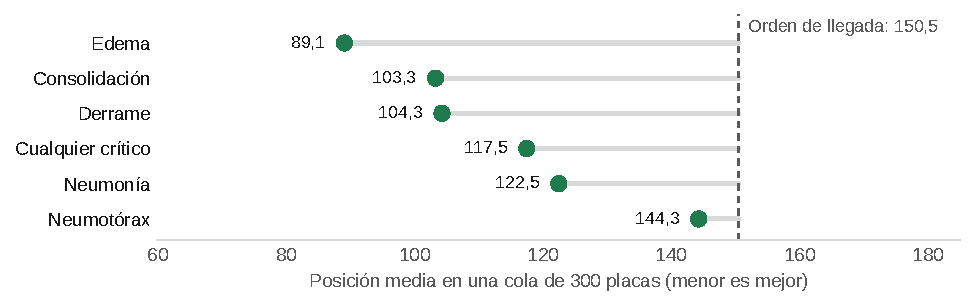
\includegraphics[width=0.94\linewidth]{figuras/cola.pdf}
\caption{Posición media de cada hallazgo en la cola priorizada.}
\end{figure}

El edema es el más favorecido: baja a la posición 89,1 y el 25,8 \% de los casos entra en las primeras 30 placas, frente al 10 \% esperado al azar. El neumotórax casi no mejora (144,3), y calibrar las salidas por percentil no lo corrigió (148,2). El AUC va de 0,614 a 0,774, por lo que el modelo sirve para priorizar con supervisión y no para decidir. No se pudo confirmar que los pesos \texttt{all} respeten la partición oficial del NIH, de modo que estos valores podrían ser optimistas.

\begin{table}[h]
\centering
\caption{Tiempo de puntuar y ordenar según el volumen, extrapolado de la medición.}
\begin{tabular}{|l|r|r|r|}
\hline
Escenario & Placas & CPU & GPU \\ \hline
Hospital de Escuintla, un día & 197 & 6,3 s & 0,8 s \\ \hline
IGSS, día promedio & 2\,455 & 1,3 min & 9,5 s \\ \hline
NIH ChestX-ray14 completo & 112\,120 & 1,0 h & 7,2 min \\ \hline
IGSS, un año de rayos X & 895\,987 & 8,0 h & 57,5 min \\ \hline
\end{tabular}
\end{table}

Para un solo hospital, la GPU no cambia la decisión clínica: la CPU ordena un día en segundos. Con una placa a la vez, la latencia fue de 45,7 ms en CPU y 13,3 ms en GPU (3,4×), ambas imperceptibles. El valor aparece a escala institucional. Un año de rayos X del IGSS pasa de un turno completo a menos de una hora (46 min con solapado), aunque esa cifra incluye estudios que no son de tórax. Esto permite volver a puntuar todo el archivo cada vez que mejore el modelo, recuperar en minutos un atraso tras una caída del sistema y, con el mismo presupuesto de tiempo, usar modelos unas 8 veces más costosos para atacar la precisión, que es hoy la limitación principal.

\section{Reproducibilidad}

El repositorio \url{https://github.com/ecarcamo/Second-CUDA-Challenge} contiene el código de las dos versiones, las pruebas, los scripts de medición, los tiempos crudos de cada corrida y este informe en LaTeX. La presentación interactiva está en \url{https://claude.ai/artifact/KvtLZwqRLCioCJeVuPnGau}, y el informe y las diapositivas en PDF están en la carpeta \texttt{entrega/} del repositorio. Para repetir el experimento desde cero:

\begin{enumerate}[leftmargin=*,itemsep=1pt,topsep=2pt]
\item \textbf{Entorno.} Se necesita Linux con una GPU NVIDIA y un driver compatible con CUDA 13, Python 3.11 y \texttt{uv}. \texttt{gpu/requirements.txt} fija las versiones exactas usadas: PyTorch 2.15.0, CuPy 14.2.0, TorchXRayVision 1.5.7, OpenCV 5.0 y NumPy 2.4.6.
\item \textbf{Datos.} \texttt{scripts/download.sh} baja las etiquetas y las particiones oficiales del espejo de Hugging Face y los cinco primeros archivos de imágenes del NIH (unos 17 GB comprimidos). Si la descarga se corta, se reanuda donde quedó.
\item \textbf{Corrida completa.} \texttt{scripts/run\_all.sh} verifica los archivos y fija la lista de 44\,999 imágenes, corre las 66 pruebas automáticas, hace una prueba corta con 500 imágenes en cada versión, barre las configuraciones de hilos de la CPU y elige la más rápida. Después mide las dos versiones oficiales y las variantes de la GPU, compara las dos colas y calcula el AUC. Un vigilante de temperatura pausa la corrida si la laptop se calienta, y cada paso ya terminado se salta, de modo que se puede retomar. En la laptop de referencia tarda unas 6 horas.
\item \textbf{Cifras y figuras.} \texttt{scripts/summarize.py} reúne todas las cifras de este informe en \texttt{resultados/RESUMEN.md}. \texttt{scripts/queue\_impact.py} repite la simulación de la cola con semilla fija y \texttt{scripts/make\_figures.py} regenera las figuras.
\end{enumerate}

Como los tiempos dependen del equipo, otra máquina dará cifras distintas, pero las colas y el AUC deben ser equivalentes.

\clearpage
\section*{Referencias}
{\setlength{\parindent}{-1.25em}\setlength{\leftskip}{1.25em}\setlength{\parskip}{3pt}

Annarumma, M., Withey, S. J., Bakewell, R. J., Pesce, E., Goh, V. y Montana, G. (2019). Automated triaging of adult chest radiographs with deep artificial neural networks. \textit{Radiology}, \textit{291}(1), 196--202. \url{https://doi.org/10.1148/radiol.2018180921}

Bradski, G. (2000). The OpenCV library. \textit{Dr. Dobb's Journal of Software Tools}.

Cohen, J. P., Viviano, J. D., Bertin, P., Morrison, P., Torabian, P., Guarrera, M., Lungren, M. P., Chaudhari, A., Brooks, R., Hashir, M. y Bertrand, H. (2022). TorchXRayVision: A library of chest X-ray datasets and models. En \textit{Proceedings of the 5th International Conference on Medical Imaging with Deep Learning} (Vol. 172, pp. 231--249). PMLR. \url{https://proceedings.mlr.press/v172/cohen22a.html}

Cosentini, R., Aliberti, S., Bignamini, A., Piffer, F. y Brambilla, A. M. (2009). Mortality in acute cardiogenic pulmonary edema treated with continuous positive airway pressure. \textit{Intensive Care Medicine}, \textit{35}(2), 299--305. \url{https://doi.org/10.1007/s00134-008-1281-7}

Harris, C. R., Millman, K. J., van der Walt, S. J., Gommers, R., Virtanen, P., Cournapeau, D., \ldots{} Oliphant, T. E. (2020). Array programming with NumPy. \textit{Nature}, \textit{585}(7825), 357--362. \url{https://doi.org/10.1038/s41586-020-2649-2}

Huang, G., Liu, Z., van der Maaten, L. y Weinberger, K. Q. (2017). Densely connected convolutional networks. En \textit{2017 IEEE Conference on Computer Vision and Pattern Recognition} (pp. 2261--2269). \url{https://doi.org/10.1109/CVPR.2017.243}

Instituto Guatemalteco de Seguridad Social. (2025). \textit{Boletín estadístico: prestaciones en salud 2024} (p. 56). \url{https://www.igssgt.org/informes-y-estadisticas/boletin-estadistico-de-salud/}

Instituto Guatemalteco de Seguridad Social. (2026, 8 de abril). \textit{Hospital del IGSS en Escuintla fortalece servicios y atención en su 64 aniversario}. \url{https://www.igssgt.org/noticias/2026/04/08/hospital-del-igss-en-escuintla-fortalece-servicios-y-atencion-en-su-67-aniversario/}

Okuta, R., Unno, Y., Nishino, D., Hido, S. y Loomis, C. (2017). CuPy: A NumPy-compatible library for NVIDIA GPU calculations. En \textit{Workshop on Machine Learning Systems (LearningSys), NIPS 2017}. \url{http://learningsys.org/nips17/assets/papers/paper_16.pdf}

Paszke, A., Gross, S., Massa, F., Lerer, A., Bradbury, J., Chanan, G., \ldots{} Chintala, S. (2019). PyTorch: An imperative style, high-performance deep learning library. En \textit{Advances in Neural Information Processing Systems 32} (pp. 8024--8035).

Wang, X., Peng, Y., Lu, L., Lu, Z., Bagheri, M. y Summers, R. M. (2017). ChestX-ray8: Hospital-scale chest X-ray database and benchmarks on weakly-supervised classification and localization of common thorax diseases. En \textit{2017 IEEE Conference on Computer Vision and Pattern Recognition} (pp. 3462--3471). \url{https://doi.org/10.1109/CVPR.2017.369}
\par}

\end{document}
